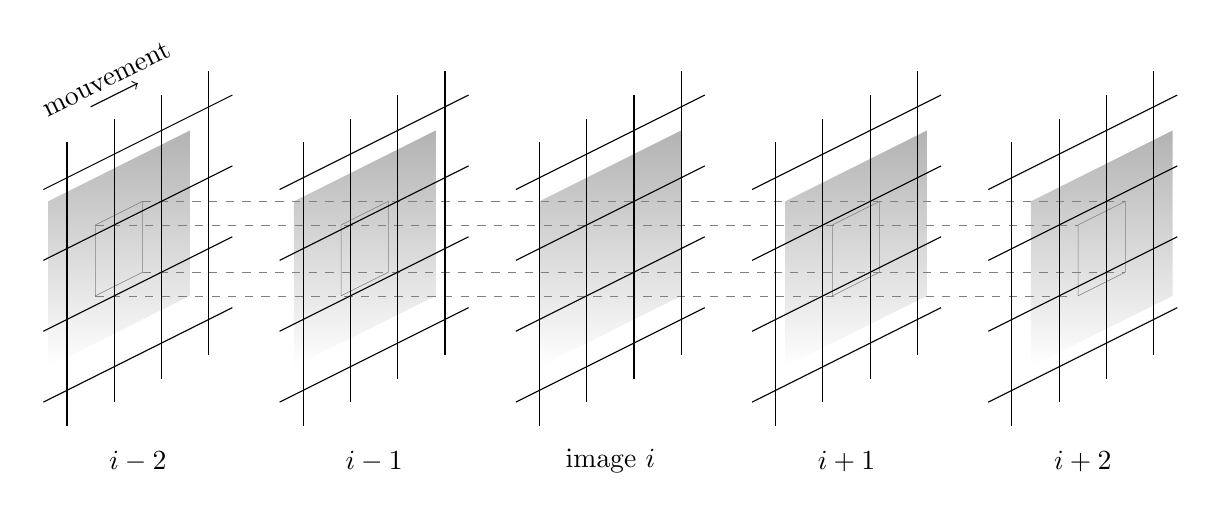
\begin{tikzpicture}[scale=0.6]

\shade[top color=black!30,shading=axis] (0.1,-4.5) -- (3.1,-3) --  (3.1,0.5) -- (0.1,-1) -- cycle;
\shade[top color=black!30,shading=axis] (5.3,-4.5) -- (8.3,-3) --  (8.3,0.5) -- (5.3,-1) -- cycle;
\shade[top color=black!30,shading=axis] (10.5,-4.5) -- (13.5,-3) --  (13.5,0.5) -- (10.5,-1) -- cycle;
\shade[top color=black!30,shading=axis] (15.7,-4.5) -- (18.7,-3) --  (18.7,0.5) -- (15.7,-1) -- cycle;
\shade[top color=black!30,shading=axis] (20.9,-4.5) -- (23.9,-3) --  (23.9,0.5) -- (20.9,-1) -- cycle;

\draw[help lines] (1.1,-3) -- (2.1,-2.5) --  (2.1,-1) -- (1.1,-1.5) -- cycle;
\draw[help lines] (6.3,-3) -- (7.3,-2.5) --  (7.3,-1) -- (6.3,-1.5) -- cycle;
\draw[help lines] (16.7,-3) -- (17.7,-2.5) --  (17.7,-1) -- (16.7,-1.5) -- cycle;
\draw[help lines] (21.9,-3) -- (22.9,-2.5) --  (22.9,-1) -- (21.9,-1.5) -- cycle;

\draw[help lines, dashed] (1.1,-3) -- (21.8,-3);
\draw[help lines, dashed] (2.1,-2.5) -- (22.9,-2.5);
\draw[help lines, dashed] (2.1,-1) -- (22.9,-1);
\draw[help lines, dashed] (1.1,-1.5) -- (21.9,-1.5);

\foreach \i in {0.25,0.75,1.25,1.75} % grille sur l'image centrale
{
	\draw (10+2*\i,\i) -- (10+2*\i,-6+\i);
	\draw (10,-3*\i) -- (14,2-3*\i);

	\foreach \j in {0,1,3,4} % grille sur les autres images
	{
		\draw (5*\j + 2*\i, \i) -- (5*\j + 2*\i, -6 + \i);
		\draw (5*\j,-3*\i) -- (5*\j + 4,2-3*\i);
	}
}

\draw[->] (1,1) -- (2,1.5) node[rotate=26.5,above,pos=0.5] {mouvement};

\draw (2,-6.5) node{$i-2$};
\draw (7,-6.5) node{$i-1$};
\draw (12,-6.5) node{image $i$};
\draw (17,-6.5) node{$i+1$};
\draw (22,-6.5) node{$i+2$};

\end{tikzpicture}
